%%
%% This is file `sample-sigconf.tex',
%% generated with the docstrip utility.
%%
%% The original source files were:
%%
%% samples.dtx  (with options: `sigconf')
%% 
%% IMPORTANT NOTICE:
%% 
%% For the copyright see the source file.
%% 
%% Any modified versions of this file must be renamed
%% with new filenames distinct from sample-sigconf.tex.
%% 
%% For distribution of the original source see the terms
%% for copying and modification in the file samples.dtx.
%% 
%% This generated file may be distributed as long as the
%% original source files, as listed above, are part of the
%% same distribution. (The sources need not necessarily be
%% in the same archive or directory.)
%%
%%
%% Commands for TeXCount
%TC:macro \cite [option:text,text]
%TC:macro \citep [option:text,text]
%TC:macro \citet [option:text,text]
%TC:envir table 0 1
%TC:envir table* 0 1
%TC:envir tabular [ignore] word
%TC:envir displaymath 0 word
%TC:envir math 0 word
%TC:envir comment 0 0
%%
%%
%% The first command in your LaTeX source must be the \documentclass command.
\documentclass[sigconf]{acmart}

\usepackage[colorinlistoftodos]{todonotes}
\usepackage{tabularx}

%%
%% \BibTeX command to typeset BibTeX logo in the docs
\AtBeginDocument{%
  \providecommand\BibTeX{{%
    \normalfont B\kern-0.5em{\scshape i\kern-0.25em b}\kern-0.8em\TeX}}}

%% Rights management information.  This information is sent to you
%% when you complete the rights form.  These commands have SAMPLE
%% values in them; it is your responsibility as an author to replace
%% the commands and values with those provided to you when you
%% complete the rights form.
\setcopyright{acmcopyright}
\copyrightyear{2021}
\acmYear{2021}
\acmDOI{}

%% These commands are for a PROCEEDINGS abstract or paper.
\acmConference[K-Cap '21]{K-Cap '21: The Eleventh International Conference on Knowledge Capture}{December 02--03, 2021}{Virtual Conference}


%%
%% Submission ID.
%% Use this when submitting an article to a sponsored event. You'll
%% receive a unique submission ID from the organizers
%% of the event, and this ID should be used as the parameter to this command.
%%\acmSubmissionID{123-A56-BU3}

%%
%% The majority of ACM publications use numbered citations and
%% references.  The command \citestyle{authoryear} switches to the
%% "author year" style.
%%
%% If you are preparing content for an event
%% sponsored by ACM SIGGRAPH, you must use the "author year" style of
%% citations and references.
%% Uncommenting
%% the next command will enable that style.
%%\citestyle{acmauthoryear}

%%
%% end of the preamble, start of the body of the document source.
\begin{document}

%%
%% The "title" command has an optional parameter,
%% allowing the author to define a "short title" to be used in page headers.
\title{OntoFlow : Easy Ontology Development Workflows for Non-technical Domain Experts}

%%
%% The "author" command and its associated commands are used to define
%% the authors and their affiliations.
%% Of note is the shared affiliation of the first two authors, and the
%% "authornote" and "authornotemark" commands
%% used to denote shared contribution to the research.
\author{Gordian Dziwis}
\authornote{}
\email{dziwis@infai.org}
\author{Lisa Wenige}
\authornotemark[1]
\email{wenige@infai.org}
\affiliation{%
	\institution{Institute for Applied Informatics}
	\streetaddress{Goerdelerring 9}
	\city{Leipzig}
	\state{Saxony}
	\country{Germany}
	\postcode{04177}
}

%%
%% By default, the full list of authors will be used in the page
%% headers. Often, this list is too long, and will overlap
%% other information printed in the page headers. This command allows
%% the author to define a more concise list
%% of authors' names for this purpose.
\renewcommand{\shortauthors}{Dziwis and Wenige et al.}

%%
%% The abstract is a short summary of the work to be presented in the
%% article.
\begin{abstract}
	For many years, the development of widely applicable and high quality ontologies has been an ongoing research topic. Among the many challenges, the lack of integrated development environments for non-technical domain experts has been one of the most pressing research challenges. But while the participation of domain experts is vital for the applicability of ontologies, there are hardly any software tools available that facilitate their active engagement. We present a solution that addresses this research gap by automating the ontology development process with the help of a workflow engine. We define a pipeline that facilitates ontology implementation, serialization, documentation and testing within the scope of a seamless automatic routine than can be easily triggered by an ontology laymen with basic knowledge of bash usage. Thus, the processing pipeline takes care of most of the operations that usually have to be taken care of by an ontology or software engineer. We demonstrate the applicability of our approach for a wide range of ontologies and provide additional results on the quality level of ontologies throughout the Semantic Web landscape.
\end{abstract}

%%
%% The code below is generated by the tool at http://dl.acm.org/ccs.cfm.
%% Please copy and paste the code instead of the example below.
%%
\begin{CCSXML}
	<ccs2012>
	<concept>
	<concept_id>10010520.10010553.10010562</concept_id>
	<concept_desc>Computer systems organization~Embedded systems</concept_desc>
	<concept_significance>500</concept_significance>
	</concept>
	<concept>
	<concept_id>10010520.10010575.10010755</concept_id>
	<concept_desc>Computer systems organization~Redundancy</concept_desc>
	<concept_significance>300</concept_significance>
	</concept>
	<concept>
	<concept_id>10010520.10010553.10010554</concept_id>
	<concept_desc>Computer systems organization~Robotics</concept_desc>
	<concept_significance>100</concept_significance>
	</concept>
	<concept>
	<concept_id>10003033.10003083.10003095</concept_id>
	<concept_desc>Networks~Network reliability</concept_desc>
	<concept_significance>100</concept_significance>
	</concept>
	</ccs2012>
\end{CCSXML}

\ccsdesc[500]{Computer systems organization~Embedded systems}
\ccsdesc[300]{Computer systems organization~Redundancy}
\ccsdesc{Computer systems organization~Robotics}
\ccsdesc[100]{Networks~Network reliability}

%%
%% Keywords. The author(s) should pick words that accurately describe
%% the work being presented. Separate the keywords with commas.
\keywords{ontologies, workflows, IDE, quality assurance}

%%
%% This command processes the author and affiliation and title
%% information and builds the first part of the formatted document.
\maketitle

\section{Introduction}

no standard toolstack in the Semantic Web community => containerisierung 
usability

\section{Related Work}
Continuous development and integration strategies have become an indispensable part of modern software engineering.
They largely consist of clean up operations, compilation of executables, application of automated tests, and the deployment of the finished application, including generation of appropriate documentation if necessary. Part of these processes is the continuous checking of any updates/ new versions as well as the triggering of troubleshooting activities if problems occur \cite{fowler}.
This ensures that software solutions are always up-to-date, that applications meet predefined quality standards and rely on stable software artifacts.\\
Likewise, in the wake of ever-growing data volumes and increased relevance of data-driven applications, effective mechanisms to control the quality-assured publication of data products have become important requirements for IT operations. Processes that follow Continuous Integration (CI) principles are equally applicable when the production of data artifacts in collaborative environments should be made more efficient. The knowledge graph community has been one of the first to adopt DevOps best practices for datasets since it heavily relies on high quality data schemas and reproducible workflows for data conversion, integration and fusion. In this line of research, several authors have proposed automated data pipelines that not only take care of data transformation but also apply quality assurance operations and automatic procedures for data publication and effective description of data artifacts
\cite{cirulli, klimek, kucera, meissner, rojas, roman, stadler, dataid}. Typically, CI mechanisms for data collections involve operations such as crawling, linking, or data transformation. These processes are usually executed automatically and, aside from the effort of creating specifications for data conversion, are little interrupted by user interactions and manual intervention. If people work with appropriate software tools in this context, they are mostly data scientists or software engineers.\\
This modus operandi differs from the determining factors in ontology development processes. The creation of an ontology usually involves several experts with diverse backgrounds and different levels of technical expertise. Therefore, an effective ontology development environment/pipeline has to foster collaboration as well as provide a graphical editor in order to effectively support development processes. By this means, even domain experts with little IT expertise can actively take part in the creation of ontologies.\\
Ontology editors such as Protégé \cite{protege}, Vocol \cite{halilaj} or WebVOWL \cite{lohmann} are already established software tools for ontology development and visualisation. Meanwhile, other applications in this area focus more on aspects of collaborative and version-based storage of ontologies so that changes can be managed decentrally and tracked over time. Software tools, such as Ontoology \cite{alobaid} or the QuitStore \cite{arndt} provide solutions for these kinds of requirements.\\
Other tools, such as Oops! focus more on the aspect of quality assurance \cite{poveda} while general purpose RDF data testing suites, such as RDFUnit \cite{rdfunit} or pySHACL\footnote{\url{https://github.com/RDFLib/pySHACL}} can be equally applied for ontology testing. Just as important as quality assurance of ontologies is documentation prepared for end users in a form understandable by users. Software applications that automatically generate ontology documentations are WIDOCO \cite{widoco}, LODE \cite{lode} or pyLODE\footnote{\url{https://github.com/RDFLib/pyLODE}}. They create a HTML representation from ontologies in standard RDF serialization formats.\\
But although software applications are already available that support collaborative ontology development processes and also automate them in parts, there is a lack of approaches as to how these processes can be linked in the sense of a CI pipeline while at the same time ensuring that laymen can actively participate in development through making changes and triggering ontology updates.
\todo{https://www.nature.com/articles/s41587-020-0439-x}

\section{Ontology Development Workflow}

- creating
- testing
- deployment

\subsection{Requirements}
The goal of Ontoflow is the best possible optimization and automation of ontology development processes which typically currently involve a great number of labor-intensive tasks, such as modeling, serialization, updating testing and documentation. Due to the fact that such development processes are carried out by several stakeholders, the workflow environment should foster a collaborative and decentralized way of working.\\
Since the development of ontologies often involves domain experts who have only limited expertise in the field of software and data engineering, OntoFlow should provide a GUI for editing the ontology, while automating the most common tasks (e.g., bash scripting and git interaction) in the background. Due to the limited IT experience of some of the involved stakeholders, it is also vital that workflows can be triggered without in-depth technical understanding of software development or semantic technologies. Reducing the amount of necessary skills for the domain expert is critical, because generally ontology development is a one time job for them. A reusable ontology workflow setup directed at domain experts helps avoiding costs for learning the involved technologies and setting up a development and hosting infrastructure (e.g., running a webserver for publishing the ontology and documentation) which - apart from working time - can incur further costs for licences and hardware. Because there is no established methodology for ontology development and it happens in diverse environments, OntoFlow must be flexible and facilitate easy modifications to accommodate for different needs.\\
Table \ref{tab:req} gives an overview of the requirements detailed in the above sections.

% Please add the following required packages to your document preamble:
% \usepackage{booktabs}
% \usepackage{multirow}
\begin{table*}[htb]
\begin{tabular}{@{}lll@{}}
\toprule
Main Requirement &
  Sub-Requirement &
  Explanation \\ \midrule
\textbf{RQ1 ODP Automation} &
  RQ1.1 Ontology serialization &
  \begin{tabular}[l]{@{}l@{}}Ontology artifacts can be automatically \\ serialized in common RDF formats \\ (e.g., RDF/XML, Turtle or NTRIPLES\end{tabular} \\\\
 & 
  RQ1.2 Ontology Validation &
  \begin{tabular}[l]{@{}l@{}}Automatic testing of ontology artifacts\\ is integrated\end{tabular} \\\\
 &
  RQ1.3 Ontology Postprocessing &
  \begin{tabular}[l]{@{}l@{}}Intgrating automatic postprocessing \\ operations, such as updating meta-information, \\ version control or diff detection\end{tabular} \\\\
 &
  \begin{tabular}[l]{@{}l@{}}RQ1.4 Ontology Publication and \\ Documentation\end{tabular} &
  \begin{tabular}[l]{@{}l@{}}Automatic deployment of ontology artifacts \\ (serialization and HTML documentation) to a server\end{tabular} \\\\
\textbf{RQ2 High (Re-)Usability} &
  RQ2.1 GUI support &
  \begin{tabular}[l]{@{}l@{}}Support of ontology modelling through \\ a GUI\end{tabular} \\\\
 &
  \begin{tabular}[c]{@{}l@{}}RQ2.2 Easy execution of ontology\\ workflows\end{tabular} &
  \begin{tabular}[c]{@{}l@{}}Domain experts (with little to no IT background)\\ should be able to trigger ontology workflows\end{tabular} \\\\
 &
  \begin{tabular}[c]{@{}l@{}}RQ2.3 Easy modification and\\ re-use of ontology workflows\end{tabular} &
  \begin{tabular}[c]{@{}l@{}}It should be easy to modify and re-use existing\\ ontology workflows\end{tabular} \\\\
\hline
\end{tabular}
\label{tab:req}
\caption{Requirements for OntoFlow}
\end{table*}
  
\subsection{Workflow Structure}

There are three possible inputs for the workflow.
Ontologies defined with the Web Ontology Language (OWL) serialized as a RDF file\todo{RDF file or RDF-file}.
Draw.io diagrams of an ontology or parts of an ontology, defined with elements from the Chowlk Ontology Visual Notation library and exported to a XML-File.

The Chowlk diagram is transformed to an OWL file and gets merged with the other OWL files.
The merged ontology is basis for the next processing steps which happen in parallel.
It is converted to different RDF serializations.
In the ontology validation process step, the ontology is validated against SHACL shapes.
For postprocessing OntoFlow picks up prov\todo{} and creates a semantic diff against the previous version.
A HTML documentation is generated.\todo{describe package}



\begin{figure}[ht]
  \centering
  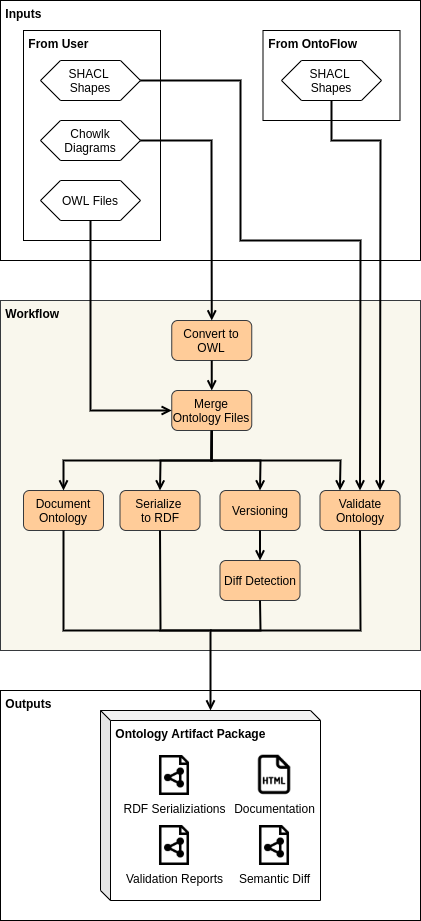
\includegraphics[width=0.35\textwidth]{workflow.png}
  \caption{Ontology Workflow}
  \label{fig2}
\end{figure}\todo{arrows, shacl shapes, tools?}\todo{screenshot of chowlk}
\begin{itemize}
  \item Ontology Development: drawing- or editor-based development 
  \item Ontology Transformation
  \item 
\end{itemize}

\subsection{Implementation and Architecture}

The architectural model for OntoFlow is a pipeline consisting of processes where each takes inputs, transform the inputs and outputs the results.
Inputs and output from the processes are interconnected.
The transformations are handled by application programs with command-line interface.
All applications are containerised and the container images are defined by an definition file.
A workflow engine manages the containers' lifecycle and executes the applications and pipes the inputs and outputs.
The pipeline process steps, with executed command\todo{}, container and connection are defined in a workflow definition file.
Those file are managed inside a version control system. There is also a ci script for building the images and pushing them to a container registry and deploying the final outputs.
The inputs are owl ontologies, chowlk diagrams and shacl shapes and output are\todo{see workflow definition} hosted in their own repository.
Workflow execution can either happen locally or in a ci environment.\todo{add benefits from architectural decisions}

The pipeline was implemented as an nextflow workflow and Docker was choosen as the container engine.
For each tool used in a process step a docker image was created, if not one already existed.
Here is a list of the used tools and their tasks:

\begin{itemize}
  \item Chowlk: Converts ontology diagram to OWL-File.
  \item pySHACL: Validates ontology against SHACL shapes.
  \item Bubastis: Creates a semantic diff to an older ontology version.
  \item Jena Riot: Serializises and merges RDF-Files.
  \item sparql-integrate: Extracts and manipulates Data in RDF-Files.\todo{versioning}
  \item pyLODE: Create ontology documentation in HTML.
\end{itemize}

Chowlk provides a library of owl diagram elements for draw.io, which is an open source diagram software.
Ontoflow can be run on any linux system with Java and Docker, it realizes it full potential in combination with the Gitlab ecosystem.
With the ontology files hosted in a Gitlab repository, the ontology can be edited collaborativly. Because draw.io can use a Gitlab repository as a storage backend collaborative editing can be achived without the user beeing exposed explicitly to git.
After a change to the ontology a Gitlab continuous integration job is triggered, which runs the workflow and publishes its resulting artifact package as an Gitlab Page.


Github also hosts Ontoflow and the tool images in its container registry.


\begin{figure}[ht]
  \centering
  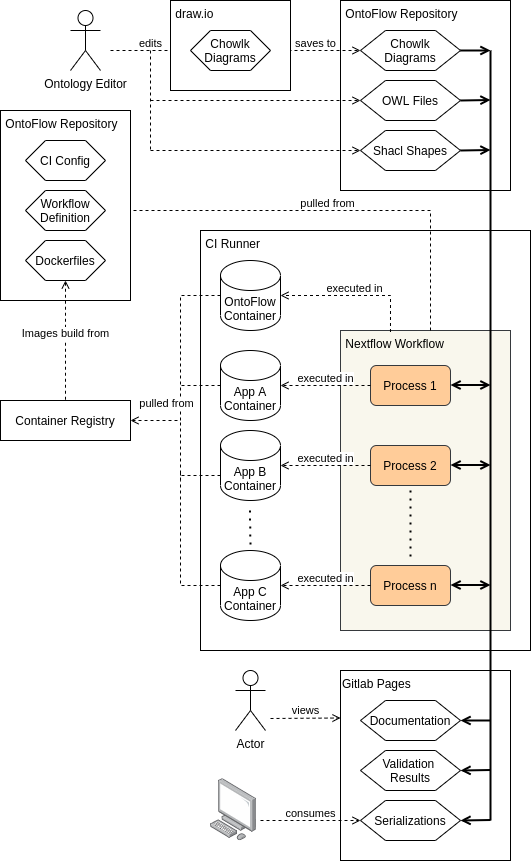
\includegraphics[width=0.45\textwidth]{architecture.png}
  \caption{Ontology Workflow}
  \label{fig2}
\end{figure}\todo{colors}

Each processes' transformation is performed
- pipline with processsteps
- put tools in containers wire together with an workflow engine and use existing infrastructure

- nextflow
- container
  - interoperabilty
  - reproducible

\section{Evaluation}

\subsection{Evaluation Setup}
- dataset description LOV (How many etc.)
- applicabilty to a broad range of ontologies 
%datasets:
%-dataset 1:  Chowlk XML collection: https://github.com/oeg-upm/Chowlk/tree/webservice/data
%-dataset 2: All ontologies from Linked Open Vocabularies (LOV), ca. 700, dumps via
%https://lov.linkeddata.es/dataset/lov/sparql
% for each of the ontologies
%=>run the entire workflow
%=>log the processing time
%log success/failure
%have a look at each processing step individually and answer the following
%questions
%how many workflows failed here?
%what was the average processing time for this workflow step?
%STEP 1: TURTLE GENERATION (dataset 1 only)
%STEP 2: DOCUMENTATION (dataset 1 & 2)
%STEP 3: SERIALIZATION (dataset 1 & 2)
%STEP 4: ONTOLOGY TESTS (dataset 1 & 2)
%for dataset 4 only: evaluate ontology tests:
%how many schema violations (owl,rdfs) where there? (rdfunit flag -s)
%how many metadata errors where there:
%=> W3C Reference:
%"One common set of additional tags that could reasonably be included here are some of the standard Dublin Core metadata tags. The subset includes those that take simple types or strings as values. Examples include Title, Creator, Description, Publisher, and Date" (W3c OWL) + owl:versionInfo
\subsection{Results}
\section{Conclusion}\todo{nfcore!!}
\section{Notes}
- follow best practices software engineering
  - github
  - linting
  - build process
  - reuse

Long term goal is that OntoFlow assumes to role package managers and build tools have for software development.\todo{also nf-core}
\bibliographystyle{ACM-Reference-Format}
\bibliography{ref}
\end{document}
\endinput
%%
%% End of file `sample-sigconf.tex'.
